\ifx\boi\undefined\ifx\problemname\undefined
\providecommand\sampleinputname{}
\providecommand\sampleoutputname{}
\documentclass[icelandic]{templates/boi}
\problemlanguage{.is}
\fi
\newcommand{\boi}{Eystrasaltsólympíuleikarnir í forritnu}
\newcommand{\practicesession}{Æfingakeppni}
\newcommand{\contestdates}{27. apríl - 1. maí, 2018}
\newcommand{\dayone}{Dagur 1}
\newcommand{\daytwo}{Dagur 2}
\newcommand{\licensingtext}{This problem is licensed under CC BY-SA 4.0.}
\newcommand{\problem}{Verkefni}
\newcommand{\inputsection}{Inntak}
\newcommand{\outputsection}{Úttak}
\newcommand{\interactivity}{Gagnvirkni}
\newcommand{\grading}{Flokkun}
\newcommand{\scoring}{Stigagjöf}
\newcommand{\constraints}{Takmarkanir}
\renewcommand{\sampleinputname}{Sýnidæmis inntak}
\renewcommand{\sampleoutputname}{Sýnidæmis úttak}
\newcommand{\sampleexplanation}[1]{Útskýring á sýnidæmi #1}
\newcommand{\sampleexplanations}{Útskýringar á sýnidæmum}
\newcommand{\timelimit}{Tímamörk}
\newcommand{\memorylimit}{Minnismörk}
\newcommand{\seconds}{s}
\newcommand{\megabytes}{MB}
\newcommand{\group}{Hópur}
\newcommand{\points}{Stig}
\newcommand{\limitsname}{Takmarkanir}
\newcommand{\additionalconstraints}{Auka takmarkanir}
\newcommand{\testgroups}{
Lausnin þín verður prófuð á einhvern fjölda prufuhópa, hver hópur gefur einhvern fjölda stiga.
Hver hópur inniheldur einhvern fjölda prufutilvika.
Til að fá stig fyrir hóp þarftu að leysa öll prufutilvik innan hópsins.
Lokastigin eru fengin úr skilunum sem gáfu hæst stig.
}
\fi
\def\version{jury-1}
\problemname{Skiptistraumur}
Fredrik er heima að leika sér með sérsmíðuðu lestarteina módeli sem hann er mjög stoltur af.
Lestarteinarnir samanstanda af $N$ hlutum sem eru tengdir í hring, númeraðir $1, 2, \dots, N$ réttsælis.
Rafstraumur í lestina fer í gegnum $M$ bogna víra sem liggja að hringnum. Hver hluti hefur að minnsta kosti einn vír við sig.

Hinsvegar hefur Fredrik fengið leið á lestinni sinni sem fer bara í hring og hefur ákveðað að bæta við 
\emph{lestrofa} á hvern hluta sem hann getur notað til að valda því að lestin fari af lestarteinunum og
í aðrar spennandi aðstæður. En rofarnir þurfa rafstraum. Ekki bara einhvern rafstraum, heldur þurfa þeir
sérstaklega \emph{skiptistraum}.\footnote{Þetta er skiljanlegt því lestarteinarnir eru sænskir -- í Svíþjóð
nota allir lestrofar (``växler'') skiptistraum (``växelström'').}
% Sorry about the terrible pun. If it translates into your language you can remove the footnote.

Fredrik hugsar að leiðin til að fá skiptistraum er að leiða rafstraum í báðar áttir.
Hver vír leiðir straum í eina átt (annað hvort réttsælis eða rangsælis) en Fredrik
ræður í hvora átt hver vír leiðir straum. Því vill hann ákveða fyrir hvern vír í hvaða
átt sá vír leiðir straum þannig að hver hluti lestarteinanna sé með réttsælis snúinn vír og rangsælis snúinn vír.

Geturðu hjálpað Fredrik?

\vspace{2mm}
%\hspace*{2mm}
\begin{center}
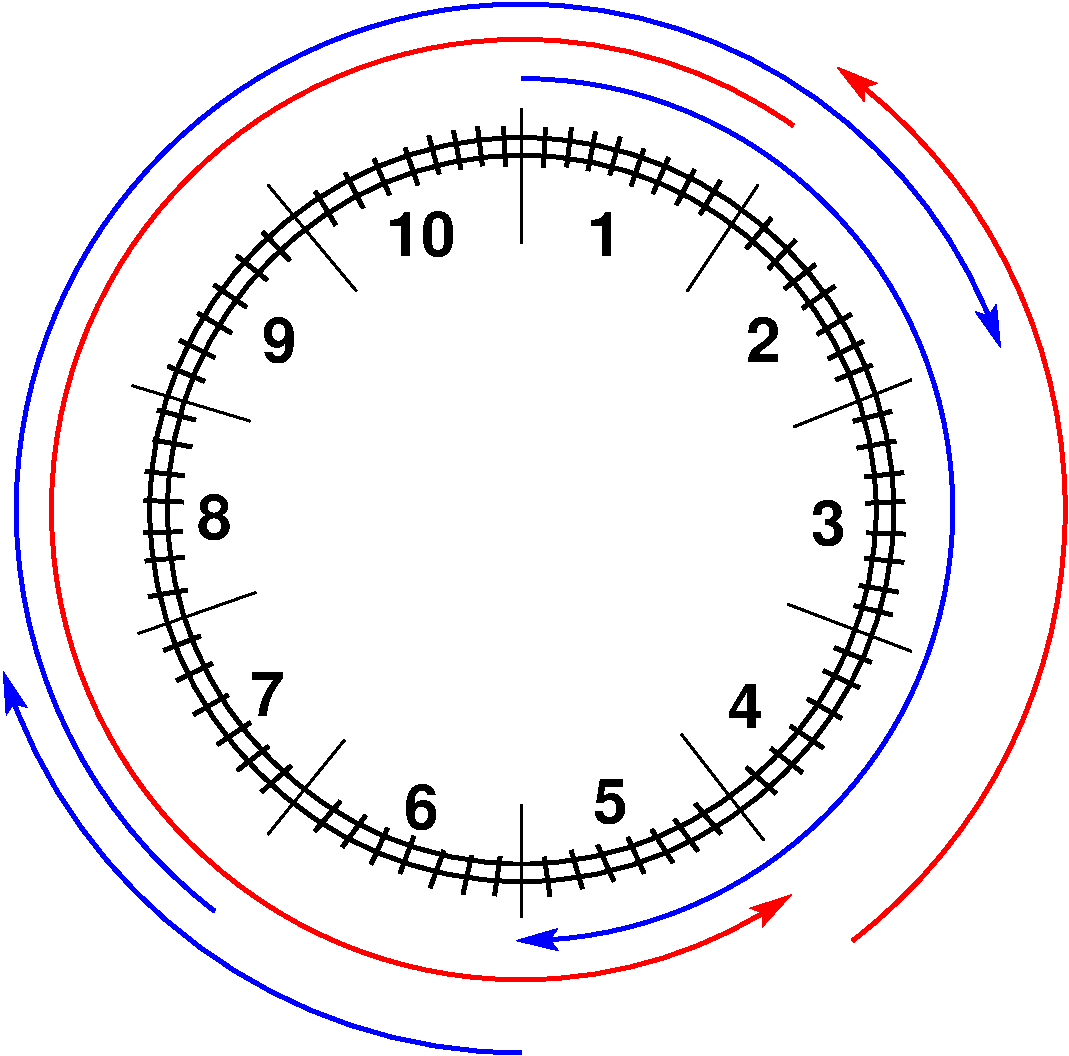
\includegraphics[width=0.5\textwidth]{alternatingfig.pdf}
\end{center}
\vspace{1mm}
{\em Lausn við fyrsta sýnidæminu. Bognu örvarnar fyrir utan teinana tákna vírana sem leiða rafstraum. Áttin sem örin bendir í táknar hvaða átt Fredrik valdi fyrir vírinn (þar sem litirnir skýra líka áttirnar). Taktu eftir að snúa má öllum örvunum við til að fá hina gildu lausnina: \texttt{11010}.}

\section*{\inputsection}
Fyrsta línan inniheldur tvær heiltölur $N$ og $M$, fjöldi hluta í lestarteinunum og fjöldi víra.

Næstu $M$ línur innihalda hver tvær heiltölur $1 \le a, b \le N$, sem þýðir að það vírinn
liggur við hluta $a, a+1, \dots, b$. Ef $b$ er minna en $a$ þá fer runan fram yfir, þ.e. hlutar $a, \dots, N, 1, \dots, b$ eru tengdir.
Taktu eftir að ef $a=b$ þá er aðeins einn hluti í rununni.

\section*{\outputsection}
Skrifaðu út línu með $M$ stöfum, hver annað hvort \texttt{0} eða \texttt{}. Stafur 
númer $i$ í línunni skal vera \texttt{0} ef straumurinn á vír númer $i$ á að streyma 
réttsælis, annars \texttt{1} ef hann á að streyma rangsælis. Ef það eru margar lausnir
til máttu skrifa út einhverja þeirra.

Ef það eru ekki til neinar gildar lausnir skaltu skrifa út ``\texttt{impossible}''.

\section*{\constraints}
\testgroups

\noindent
\begin{tabular}{| l | l | l | l |}
\hline
\textbf{\group} & \textbf{\points} & \textbf{\limitsname} & \textbf{\additionalconstraints} \\ \hline
  1     & 13     & $2 \le N, M \le 15$ & \\ \hline
  2     & 20     & $2 \le N, M \le 100$ & \\ \hline
  3     & 22     & $2 \le N, M \le 1000$ & \\ \hline
  4     & 19     & $2 \le N, M \le 100\,000$ & Enginn vír er þannig að $b < a$. \\ \hline
  5     & 26     & $2 \le N, M \le 100\,000$ & \\ \hline
\end{tabular}

